%% fundamentals.tex
The biological neuronal system initially inspired neural networks.
Accordingly, \secref{neurons} explains how biological neurons and learning work and relates them to their artificial counterparts.
Next, \secref{ann}  describes artificial neural networks, connecting many artificial neurons.
In \secref{limitationsDL}, the limitations of such artificial neural networks are pointed out.
Finally, \secref{neurocomputing} explores biologically more plausible learning methods.
These last two sections are not crucial for comprehending this thesis and can optionally be skipped. However, they are relevant for future work (i.e. to answer the question of how the proposed framework could be further improved) and serve as supplementary material for interested readers seeking a more comprehensive overview of the entire field.

\section{Human Brain}\seclbl{neurons}
\begin{figure}[h]
    \centering
    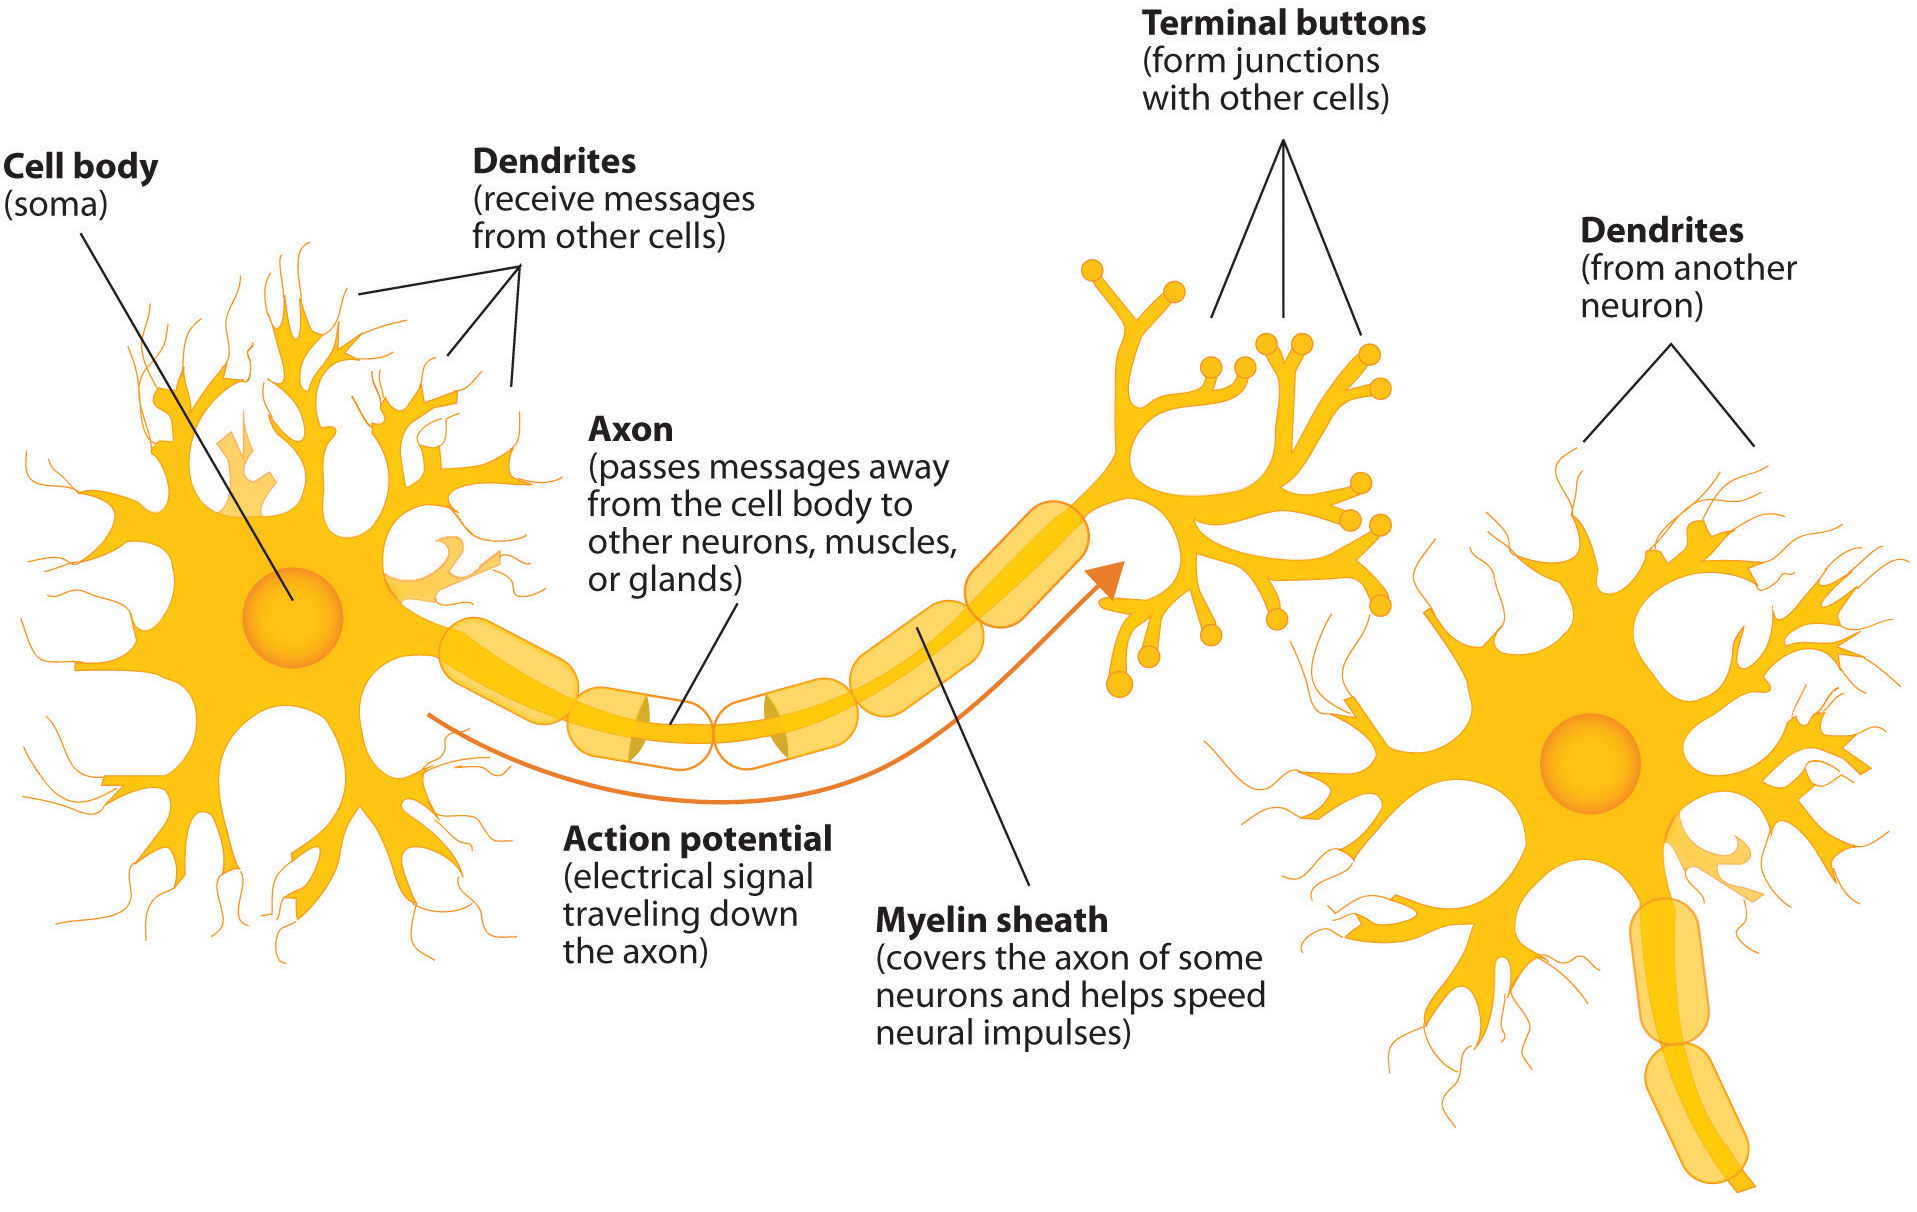
\includegraphics[width=0.99\textwidth]{components_of_neuron}
    \caption[Diagram of the components of a biological neuron]{A diagram of the components of a biological neuron. The image is from \citeay{wikipedia_neuron_2023}.}
    \figlbl{components_neuron}
\end{figure}

A biological neuron is a cell that communicates with other neurons through synapses, as illustrated in \figref{components_neuron}.
Communication takes place through precisely timed electrical pulses called spikes or action potential.
Biological neurons are electrically excitable by voltage changes across their membranes.
The neuron generates an action potential if the changes are significant enough within a short interval.
This action potential propagates along the axon, activating synaptic connections with other neurons.
The synaptic signal can be excitatory \sidecite{takagi_roles_2000} or inhibitory \sidecite{coombs_specific_1955}, making the postsynaptic neuron more or less likely to fire an action potential itself.
However, biological neurons do not follow strict rules; they adapt their firing rate to constant inputs, may continue firing after an input signal disappears and can even fire when no input is active \cite{wilson_spontaneous_1981, diamond_identifying_2019}.

Biological neurons can be classified into sensory neurons, motor neurons, and interneurons.
Sensory neurons respond to external stimuli such as light or sound and send signals to the spinal cord or the brain.
Motor neurons receive brain and spinal cord signals to control muscles or organs.
Interneurons establish connections between neurons within the same brain or spinal cord region.
However, this classification is a simplification, as the human brain consists of approximately 100 billion neurons \sidecite{herculano-houzel_human_2009} with diverse molecular, morphological, connectional, and functional properties \sidecite{zeng_neuronal_2017}.

Inspired by biological neurons, several variants of artificial neurons have been proposed in the literature and are discussed in \secref{ann}.
However, artificial neurons are simplified models compared to their biological counterparts, ignoring much complexity. Like biological neurons, artificial neurons are usually connected to other neurons and form an artificial neural network. Although the neurons in the first layer of an artificial network could be considered sensory neurons, the neurons in the last layer could be considered motor neurons, and the neurons in the middle layer could be considered interneurons, this distinction is less meaningful because artificial neurons function similarly regardless of their position, except for variations in their activation function (c.f. \secref{ann}).

Furthermore, artificial neural networks (ANNs) have a simpler organisational structure than the human brain. ANNs typically consist of one or a few network parts, such as encoders, which map data to a latent space, and decoders, which convert data from the latent space into a target vector. Each layer serves a different purpose, with earlier layers extracting low-level features and later layers combining them into higher-level latent representations. However, ANNs are considered monolithic because they are hierarchical and typically trained in an end-to-end fashion \sidecite{glasmachers_limits_2017}. In contrast, the human brain consists of many interconnected organisational units, each responsible for a specific function. For example, in the cerebral cortex, which is responsible for vision, there exist numerous small sub-units dedicated to specific tasks as illustrated in \figref{visual_cortext}. Furthermore, the human brain does not comprise an organisational hierarchy as ANNs. In the human brain, each unit applies similar deterministic functions to the information it receives. Furthermore, the biological network in the human brain is dynamic and subject to change through growth and reorganisation, known as neuroplasticity or neuronal plasticity \sidecite{costandi_neuroplasticity_2016}.

In addition to the structural and functional differences, biological and artificial networks differ in their learning strategies.
An artificial learning system requires a feedback signal from which it can learn.
This is called the \emph{credit assignment problem}.
Backpropagation of error (c.f. \secref{ann}) is the state-of-the-art algorithm that solves this problem by propagating the error signals back through the network \sidecite{rumelhart_learning_1986}.
However, information in the brain flows only in one direction, from presynaptic to postsynaptic neurons.
Therefore, backpropagation of error is not biologically plausible.
Furthermore, the brain relies on localised learning \sidecite{lillicrap_backpropagation_2020}, where each unit adapts its behaviour based on the information it receives.
The actual biological learning algorithm remains unknown. Evidence suggests that the brain learns by connecting cells that are active at the same, which can be implemented with the Hebbian learning algorithm \sidecite{hebb_organization_1949}.
Researching biologically more plausible learning algorithms for artificial neural networks is a hot research topic summarised in \secref{alt_train_algo}.

\begin{figure}[h]
    \centering
    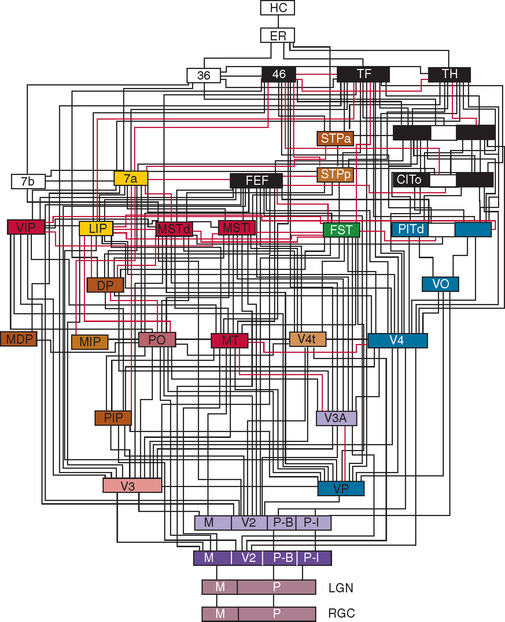
\includegraphics[width=0.89\textwidth]{felleman_visual_cortex}
    \caption[Organisation of the visual system in the cerebral cortex]{The organisation of the visual system in the cerebral cortex. The image is from \citeay{felleman_distributed_1991}.}
    \figlbl{visual_cortext}
\end{figure}

Thus, among the most important differences between biological and artificial neurons is the time-dependent and asynchronous firing of biological neurons compared to the predefined synchronous firing of artificial neurons. In addition, biological networks have different types of neurons and rely on local learning, while artificial networks usually comprise identical neurons and utilise a global error correction algorithm. Finally, biological networks are organised in a complex way \sidecite{felleman_distributed_1991}, while artificial networks are composed of simpler connection patterns.

Biological findings highly inspire the proposed vision framework.
Since biological systems still have many advantages compared to their artificial counterpart, especially the differences between these systems are of interest and could be promising in developing novel architectures.
Therefore, \secref{framework_neuroscience} dives deeper into biological principles, identifies central concepts of the human's vision system, and transfers them to a computational framework.

\section{Artificial Neural Networks}\seclbl{ann}
McCulloch and Pitts \sidecite{mcculloch_logical_1943} proposed the first model of a neuron that can be connected to other neurons.
Similar to the biological neuron, the artificial neuron of McCulloch and Pitts receives multiple input signals and transforms them into an output signal.
Their neuron takes a binary input vector $\boldsymbol{x} = (x_1, ..., x_n)$ where $x_i \in \{0, 1\}$ and maps it to an output $\hat{y} \in \{0, 1\}$.
The mapping from the input to the output is done by using an aggregation function $g(\boldsymbol{x})$ that sums up the input vector $\boldsymbol{x}$ and an activation function $f(z)$ that outputs $1$ if the output $z = g(\boldsymbol{x})$ is bigger than a threshold $\theta$ and $0$ otherwise.
%
\begin{align}\eqlbl{McCulloch_Pitts_agg}%
	z &= g(\boldsymbol{x}) = g(x_1, ..., x_n) = \sum_{i=1}^{n}x_i\\
		\hat{y} &= f(z) = \begin{cases}
      		1, & \text{if}\ z \geq \theta \\
      		0, & \text{otherwise}
    	\end{cases}
\end{align}
%
The formula is often rewritten by using a positive  bias $b$ term instead of the  threshold $\theta$
%
\begin{align}\eqlbl{McCulloch_Pitts_agg}%
	z &= g(\boldsymbol{x}) = g(x_1, ..., x_n) = \sum_{i=1}^{n}x_i + b\\
		\hat{y} &= f(z) = \begin{cases}
      		1, & \text{if}\ z \geq 0 \\
      		0, & \text{otherwise}
    	\end{cases}
\end{align}
%
In 1958, \sideciteay{rosenblatt_perceptron_1958} proposed the perceptron, which extends the neuron with learnable bias with additional learnable weights: The input vector $\boldsymbol{x}$ of length $n$ is multiplied with a weight vector $\boldsymbol{w} \in \mathbb{R}^n$ of the same length.
%
\begin{align}\eqlbl{nn}%
	z = g(\boldsymbol{x}) = \boldsymbol{w} \cdot \boldsymbol{x} + b = \left( \sum_{i=1}^{n}w_i \cdot x_i \right) + b
\end{align}
%
The weight vector $\boldsymbol{w}$ remains identical if the output $\boldsymbol{\hat{y}}$ corresponds to the desired output $\boldsymbol{y}$ or is adjusted otherwise (c.f. \secref{learning_algorithm}). Later, the activation function \(f(z)\) was replaced with other functions so that the output can also be a real number \(\hat{y} \in \mathbb{R}\) \sidecite{fukushima_visual_1969}. Often-used activation functions are
%
\begin{align}\eqlbl{act_functions}%
		\text{Sigmoid: } & f(z) = \sigma(z) = \frac{1}{1+\mathrm{e}^{-z}}\\
		\text{Rectified linear unit (ReLU): } & f(z) = (z)^{+} = \max\{0, z\}\\
		\text{Hyperbolic tangent (tanh): }  & f(z) = \tanh(z) = \frac{\mathrm{e}^{z}-\mathrm{e}^{-z}}{\mathrm{e}^{z}+\mathrm{e}^{-z}}
\end{align}


To summarise, compared to their biological counterparts, artificial neurons exhibit non-temporal behaviour and output continuous values instead of discrete binary spikes. Neurons with time-dependent spike patterns are computationally inefficient on current hardware and encounter difficulties in converting static inputs into time-based signals, which precludes their use in the framework proposed in this thesis. In contrast, binary neurons are highly robust against noise \sidecite{akhtar_threat_2018} and interpretable as they typically turn on if a specific feature is present and off otherwise \sidecite{gross_genealogy_2002}.
Consequently, the proposed framework leverages the robustness of binary neurons but does not utilise time dependency.


\subsection{Fully Connected Layer}\seclbl{fully_connected_layer}
Artificial neural networks (ANNs) consist of several neurons organised in a network. These neurons are arranged in layers. In a basic configuration, each neuron in one layer is connected to each neuron in the following layer, forming a so-called fully connected layer (FC).

In a fully connected layer with $k$ neurons, the input $\boldsymbol{x} \in \mathbb{R}^n$ is multiplied with a weight matrix $\boldsymbol{W} \in \mathbb{R}^{n\times k}$ and a bias $\boldsymbol{b} \in \mathbb{R}^k$ is added to obtain the layer's output $\boldsymbol{\hat{y}} \in \mathbb{R}^k$.
\begin{align}\eqlbl{nn3}%
	\boldsymbol{z} = \boldsymbol{W} \cdot \boldsymbol{x} + \boldsymbol{b}
\end{align}
\begin{align}
	\hat{\boldsymbol{y}} = f(\boldsymbol{z})
\end{align}
%
The universal approximation theorem \sidecite{cybenko_approximation_1989} states that a shallow network with one hidden layer (i.e. one layer between input and output layer) and enough neurons can approximate any mapping function between inputs and outputs.
However, a sequential arrangement of multiple layers is more efficient for complex functions. This hierarchical approach allows the network to learn a hierarchy of features and capture intricate patterns \sidecite{bengio_deep_2012}.

In a multi-layer perceptron (MLP) with $L$ layers, the input \(\boldsymbol{x}\) is passed through each layer, whereby each subsequent layer \(l\) uses the output of the previous layer \(l-1\) as input.
The layers in the network are denoted with a superscript square bracket notation, where $l$ is the layer index. 
For instance, the weights of layer $l$ are denoted as $\boldsymbol{W}^{[l]}$, the bias as \(\boldsymbol{b}^{[l]}\), the output of the aggregation function as \(\boldsymbol{z}^{[l]}\), and the output of the activation function as \(\boldsymbol{a}^{[l]}\)\sidenote{Hereafter, the intermediate layer outputs are denoted as $\boldsymbol{a}^{[l]}$, while $\boldsymbol{\hat{y}}$ is used for the model's final output of the last layer.}.
The input in the first layer is the input data itself, i.e. $\boldsymbol{a}^{[0]} = \boldsymbol{x}$, and the output of the last layer corresponds to the model's prediction, denoted as $\boldsymbol{a}^{[L]} = \hat{\boldsymbol{y}}$. With this denotation, the mathematical formulation of an MLP can be defined as follows:
%
\begin{align}\eqlbl{mlp}
		\boldsymbol{z}^{[l]} = \boldsymbol{W}^{[l]}\boldsymbol{a}^{[l-1]} + \boldsymbol{b}^{[l]}
\end{align}
%
\begin{align}\eqlbl{mlp2}
		\boldsymbol{a}^{[l]} = f(\boldsymbol{z}^{[l]})
\end{align}

As outlined in \secref{intro_motivation}, layer-wise data processing leads to early commitment. Within the context of this thesis's framework, additional intra-layer connections, so-called lateral connections, are introduced. Combined with a local learning algorithm, these connections allow the model to attend to local and global features simultaneously.


\subsection{Learning Algorithm}\seclbl{learning_algorithm}
The model's prediction $\boldsymbol{\hat{y}}$ will only be close to the target output $\boldsymbol{y}$ if the weights $\boldsymbol{W}^{[l]}$ and biases $\boldsymbol{b}^{[l]}$ are properly defined in every layer $l$.
These parameters are learned through training, typically using backpropagation of errors \sidecite{rosenblatt_principles_1962, linnainmaa_taylor_1976}.
Training can take place in a supervised, unsupervised, semi-supervised or reinforcement learning setting \cite{russell_artificial_2021, simmler_survey_2021}. In supervised learning \cite{cord_supervised_2008}, the model output $\boldsymbol{\hat{y}}$ is compared to a target output $\boldsymbol{\hat{y}}$. Self-supervised (also called unsupervised) learning \cite{liu_self-supervised_2021} finds patterns in input data without predefined labels. Typically, the target $\boldsymbol{y}$ is derived from the data automatically, for example, by predicting a masked part of the data. Semi-supervised learning \cite{van_engelen_survey_2020} combines labelled and unlabelled data. Lastly, reinforcement learning algorithms \cite{arulkumaran_deep_2017} aim to maximise the rewards they receive from environments based on their actions.

All these learning principles have in common that a loss function \cite{wang_comprehensive_2022} (also called an objective function) $\mathcal{L}(\boldsymbol{\hat{y}}, \boldsymbol{y})$ is used to calculate the goodness of the model output $\boldsymbol{\hat{y}}$ relative to the target output $\boldsymbol{y}$.
The selected loss function is minimised iteratively using stochastic gradient descent (SGD)\sidenote{There also exist other optimisation algorithms such as SGD with momentum, RMSprop or Adam \cite{kingma_adam_2017}.}. This process continues until the network reaches a (local) minimum.
Stochastic gradient descent is based on the insight that the negative gradient of the loss value indicates the direction of the steepest descent, i.e. the direction in which the loss decreases the most. Consequently, SGD updates the parameters of the network by taking steps of size $\eta$ (the learning rate) in the direction of the negative gradient:
%
\begin{align}\eqlbl{sgd}
	\begin{aligned}
		\Delta \boldsymbol{W}^{[l]} = & -\eta \cdot \left( \nabla_{\boldsymbol{W}^{[l]}} \mathcal{L} \right)\\
		\boldsymbol{W}^{[l]} \coloneqq & \boldsymbol{W}^{[l]} + \Delta \boldsymbol{W}^{[l]}
	\end{aligned}
\end{align}
%
and
%	
\begin{align}\eqlbl{sgd2}	
	\begin{aligned}
		\Delta \boldsymbol{b}^{[l]} = & -\eta \cdot \left( \nabla_{\boldsymbol{b}^{[l]}} \mathcal{L} \right)\\
		\boldsymbol{b}^{[l]} \coloneqq & \boldsymbol{b}^{[l]} + \Delta \boldsymbol{b}^{[l]}
	\end{aligned}
\end{align}
%
The term $\left( \nabla_{\boldsymbol{W}^{[l]}} \mathcal{L} \right)$ is the gradient of the weights $\boldsymbol{W}^{[l]}$  with respect to the loss $\mathcal{L}(\cdot)$ and the term $\left( \nabla_{\boldsymbol{b}^{[l]}} \mathcal{L} \right)$ is the gradient of the bias \(\boldsymbol{b}^{[l]}\)  with respect to $\mathcal{L}(\cdot)$.
The gradients of the weights can efficiently be calculated with backpropagation of error \sidecite{rosenblatt_principles_1962, linnainmaa_taylor_1976}, which is, in fact, just an intelligent implementation of the chain rule\sidenote{While a detailed discussion of backpropagation is out of scope for this thesis, we refer interested readers to the book ``Understanding Deep Learning'' by \citeay{prince_understanding_2023}}.

Using a global error correction algorithm such as backpropagation of error optimises consistency at a single point in the network, i.e. between                                              mn\boldsymbol{y}



\subsection{Convolutional Networks}\seclbl{cnns}
In \secref{fully_connected_layer}, fully connected layers are discussed.
However, a problem with fully connected layers is that they are not position invariant, meaning they cannot recognize patterns regardless of their location in the input.
Convolutional neural networks (CNNs) \sidecite{fukushima_neocognitron_1980, waibel_phoneme_1987, lecun_backpropagation_1989} are inspired by biological processes \sidecite{hubel_receptive_1968, fukushima_neocognitron_2007} and can overcome this limitation: CNNs exhibit position invariance and are capable of extracting local features that are abstracted in a hierarchically.
Like fully connected networks, a CNN comprises an input layer, an output layer, and multiple hidden layers in between.
A typical CNN consists of subsequently connected convolutional layers and pooling layers.
Usually, an activation function is applied after each convolutional layer, while no activation function is used after pooling layers.

Convolutional layers employ convolution filters or kernels that slide along the input, generating translation-equivariant \sidecite{gerber_stride_2020} responses known as feature maps \sidecite{zhang_parallel_1990}.
Translation-equivariant means that the relative placement of objects remains consistent between the layer's input and output, as the same filter is applied to all image positions.
During the filtering process, the dot product is calculated between the filter and an input area (of the same size as the filter), resulting in a scalar value that is assigned to one position of the output matrix (i.e. the feature map) \cite{goodfellow_deep_2016}.
This process is repeated by shifting the filter by a specified stride until the entire input is processed and all values in the output matrix are calculated.
Compared to fully connected layers of the same size, convolutional layers require much fewer parameters because only the kernels need to be learned.
This process of re-using the same weights at different input locations is known as parameter sharing \cite{gerber_stride_2020}.
By stacking multiple layers, CNNs become hierarchical: The convolutional operation squeezes information from surrounding pixel into a single output cell. Thus, using multiple layers sequentially continuously enlarges the receptive field - —the area of input pixels that can influence a single value in a layer's feature map \sidecite{bengio_deep_2012}.

Pooling layers downsize the input rather than extracting features \cite{ciresan_flexible_2011}.
Similar to convolutional layers, they slide a filter along the input.
However, unlike convolutional layers, pooling filters do not have learned parameters but use an aggregation function.
Usually, the filter selects the pixel with the highest value (max pooling) or calculates the average (average pooling) within the considered input area and uses this value as output.
The filter is then shifted by its size, ensuring that non-overlapping patches of the image are processed.
Pooling layers discard a considerable amount of information but effectively reduce complexity and improve the model's robustness \cite{ciresan_flexible_2011}.

\begin{figure}[h]
    \centering
    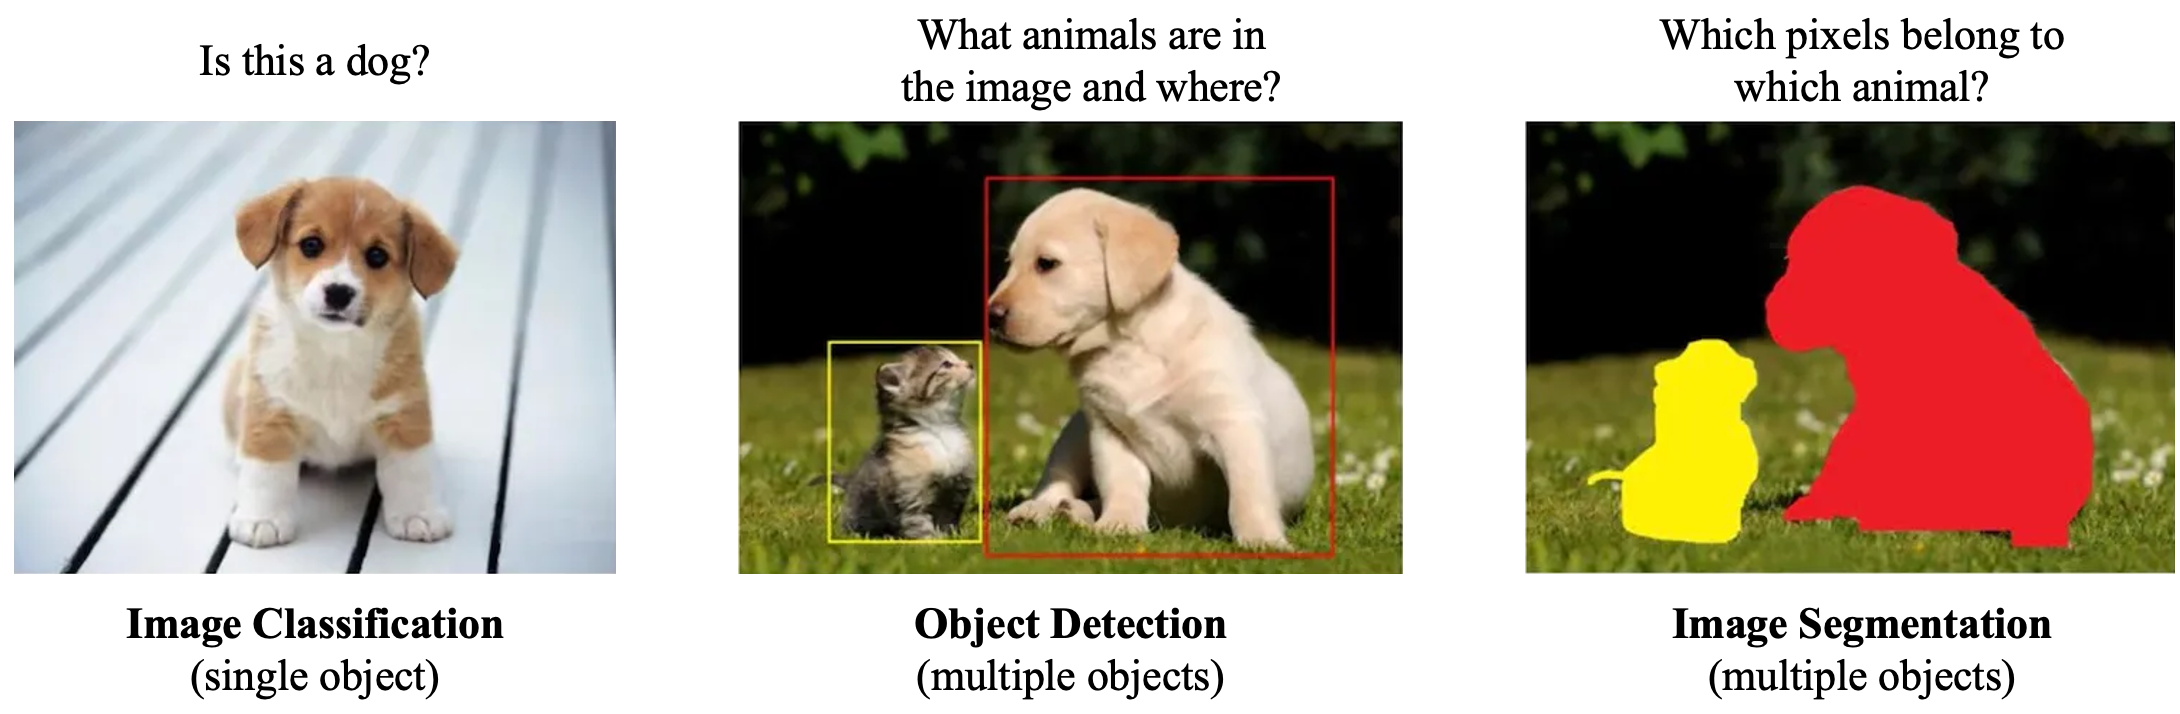
\includegraphics[width=0.99\textwidth]{image_analysis}
    \caption[Overview of different image analysis tasks]{Overview of different image analysis tasks. The image is taken from \citeay{venture_beat_new_2023} and slightly adapted.}
    \figlbl{img_analysis_tasks}
\end{figure}
In recent decades, various CNN architectures have been proposed, usually consisting of different combintations of convolutional and pooling layers. Besides using different network parameters, the performance can be further improved by adding parallel processing paths \cite{szegedy_going_2015}, batch normalisation \cite{ioffe_batch_2015}, or skip connections \cite{he_deep_2016}. Furthermore, CNNs can be utilized for different tasks such as image classification (predict image-level labels) \cite{schmarje_survey_2021}, object detection (predict a bounding box) \cite{zou_object_2023}, or semantic segmentation (predict pixel-level labels) \cite{asgari_taghanaki_deep_2021}. An overview of these tasks is provided in \figref{img_analysis_tasks}.

Compared to fully linked layers, CNNs are able to recognise patterns at different positions in the input without explicit training due to the use of shifting kernels. However, CNNs are still not fully translation invariant \cite{gerber_stride_2020}. Moreover, valuable information is lost to the pooling layers in CNNs, such as the exact positions and properties of features \cite{ciresan_flexible_2011}. Discarding valuable information can also be the reason for misclassification \sidecite{sharma_implications_2019}.

Besides CNNs, alternative architectures for image processing have emerged that are characterised by position invariance, such as the vision transformer (ViT) \sidecite{dosovitskiy_image_2021} or MLP mixer \sidecite{tolstikhin_mlp-mixer_2021}. However, providing an in-depth description of these architectures would exceed the scope of this introduction to deep learning.


\section{Limitations}\seclbl{limitationsDL}
\paragraph{Computing Resources.} Deep learning models are typically trained on modern computing infrastructure. They take advantage of Moore's law \sidecite{moore_cramming_1965}, which states that the number of transistors in a dense integrated circuit doubles about every two years. However, the physical limits of transistor size will most likely stop this exponential growth \sidecite{kumar_fundamental_2015}, and the future progress of hardware remains uncertain.
Alongside the growth in computing power, the size of modern deep learning models has also exhibited exponential growth:
For example, state-of-the-art language models have experienced astonishing growth in the number of parameters in the past years: In 2018, ELMo used around 94 million parameters \sidecite{peters_deep_2018}, in 2020, GPT-3 used around 175 billion \sidecite{brown_language_2020}, and in 2022, Megatron-Turing NLG 530B has 530 billion parameters \sidecite{smith_using_2022}.
An analysis by \citeay{open_ai_ai_2018} shows exponential growth in computational usage by AI models, with a doubling time of about 3.4 months, outpacing the rate of hardware progress, which has a doubling time of 2 years. Moreover, the increasing size of deep networks poses a challenge for inference on low-budget hardware such as smartphones or embedded systems \sidecite{berthelier_deep_2021}. Although techniques such as quantisation \sidecite{wu_integer_2020}, model pruning \sidecite{choudhary_comprehensive_2020} and model distillation \sidecite{zhou_distilling_2021} exist to reduce model size after training, the question is whether increasing model size is the best way to develop more advanced systems regarding feasibility but also regarding energy consumption \cite{garcia-martin_estimation_2019}.

\paragraph{Catastrophic Forgetting.} Another major issue of deep learning systems is that they suffer from catastrophic forgetting \cite{kirkpatrick_overcoming_2017, liu_overcoming_2021}.
If a model is trained on a specific task and afterwards trained (or fine-tuned) on another task, the model suffers a ``catastrophic'' drop in performance over the first task.
The reason for this effect is that during training on the second task, the model adjusts the parameters learned during the first task and, therefore, ``forgets'' the learned mapping functions.
Mixing all datasets or learning all tasks in parallel in a multi-task setting \sidecite{zhang_survey_2022} does not seem feasible to achieve general intelligence as general intelligence might require training on many unrelated tasks. Therefore, models should not forget previously learned knowledge even if a new task is learned.
Catastrophic forgetting is also caused by the fact that learning is mostly done offline\sidenote{Offline in this context means that the model parameters are not adapted after training during inference time.}.
Online learning \sidecite{sahoo_online_2018} and lifelong learning \sidecite{parisi_continual_2019} are hot research topics.
However, these methods still need to be established. Moreover, such models do not solve catastrophic forgetting but can only adapt better to changing conditions.

\paragraph{Extrapolate Data Distribution.} It is questionable if deep learning models can achieve \emph{real} generalization\sidenote{Generalisation refers to the ability of the model to adapt appropriately to previously unseen data from the same distribution.} in the current learning framework.
With enough data, deep learning can achieve generalisation in the sense that the model can interpolate within the known data distribution.
However, deep learning models fail to extrapolate.
For example, convolutional neural networks (CNNs) do not generalise to different viewpoints unless added to the training data \sidecite{madan_when_2022}.
The reason is that the networks are optimized to learn a model of observed data and typically have a high degree of freedom (i.e. many parameters).
Thereby, they tend to learn (too) complex models of the data: For example, modern language models have up to 530B floating-point parameters \cite{smith_using_2022}, while the human brain has 100B binary neurons in total \cite{herculano-houzel_human_2009}.
Furthermore, such artificial networks do not reason about the learned model. For example, humans believed for thousands of years in the geocentric model (the earth is in the centre of the universe) until the heliocentric model (the sun is in the centre) superseded it. Artificial networks lack this ability to reason about the best model for observed data. Instead, they tend to make small adjustments to the existing model until it no longer improves.

\paragraph{Data Hunger.} Deep learning cannot learn abstract relationships in a few trials but requires many samples and is thus data-hungry.
Gary Marcus \sidecite{marcus_deep_2018} showcased this problem with an example: He defines the new word ``schmister'' as a sister over the age of 10 but under the age of 21. He found that humans can immediately infer whether they or their best friends have any ``schmister''. However, modern deep learning systems lack a mechanism for learning abstractions through explicit, verbal definitions and require thousands or even more training samples\sidenote{LLMs can deal with such definitions when they are put into the context during inference but not when the example is only shown once during training.}.

\paragraph{Casual Reasoning.} No deep learning model has been able to demonstrate causal reasoning generically.
Deep learning models find correlations between input and output data but not causation \cite{prince_understanding_2023}.
Other AI approaches, such as hierarchical Bayesian computing \cite{allenby_hierarchical_2005} or probabilistic graphical models \cite{koller_probabilistic_2009} are better at causal reasoning but do not work well for processing high-dimensional data.

\paragraph{Embodiment.} Deep learning models are, to some extent, too isolated since they have no embodiment and cannot interact with the world.
For example, the human body provides needs, goals, emotions, and gut feelings, One could argue that the body is, therefore, even a co-processor of the brain.
In current deep learning systems, emotions are absent, and the goals are set externally.
Deep reinforcement learning \cite{dong_deep_2020} is a first step toward dissolving this isolation as the models (called agents) interact with a virtual environment. 
However, AI systems interacting with the real world have not worked well so far.
Moravec's paradox from 1995 \sidecite{moravec_mind_1995} states that ``it is comparatively easy to make computers exhibit adult level performance on intelligence tests or playing checkers, and difficult or impossible to give them the skills of a one-year-old when it comes to perception and mobility''.
This statement still seems true almost $30$ years later.


\section{Neurocomputing}\seclbl{neurocomputing}
Neuroinformatics is a recognised subfield of neuroscience that focuses on implementing learning algorithms that adhere to biological plausibility. As a result, researchers are addressing the discrepancy described in \secref{neurons} and striving to develop alternative learning algorithms.

\subsection{Hebbian Learning}\seclbl{hebbian}
Hebbian learning, as proposed by \sideciteay{hebb_organization_1949}, implements the adaptive nature of the connections between cells in the nervous system. Hebb's description states that when an axon of cell A is in close proximity to cell B and consistently contributes to its firing, growth processes or metabolic changes occur in one or both cells that increase the effectiveness of cell A in firing cell B. This description is often summarised as ``neurons that fire together wire together''.

Hebbian learning describes the update of the synaptic weight $w_{ij}$ connecting neuron $i$ to neuron $j$. The weight change depends on the presynaptic activity $a_i$ of neuron $i$ and postsynaptic activity $a_j$ of neuron $j$. The presynaptic and postsynaptic activity corresponds to the output resulting from a neuron's activation function $f(\cdot)$ in the preceding and following layers, respectively.
%
\begin{align}\eqlbl{hebb_1}
	\Delta w_{ij} = \eta a_i a_j
\end{align}
%
where \(\eta\) is the learning rate.
In a binary context, the weights between frequently co-activated neurons increase, a process known as Hebbian plasticity.
This rule causes two cells or cell sub-networks that are constantly active together to form an ``association'' where the activation of one cell or system promotes the activation of the other.
When a system receives inputs that generate a recurring pattern of activity, the group of active cells comprising that pattern gradually strengthens their connections. Consequently, when a group of neurons that represent a specific pattern is active, they tend to activate all neurons typically associated with this pattern. In this thesis, I call this effect \emph{lateral support}.

The aforementioned Hebbian rule increases the weight between two binary cells that are active together and does not change when only one or none of the cells fires. Thus, the connection can only grow stronger.
However, synaptic signals in the human brain can also be inhibitory \cite{coombs_specific_1955}.
In the context of Hebbian learning, inhibition is interpreted as decreasing the weight between cells that fire exclusively.
Therefore, inhibition can be implemented by leveraging the covariance of neuronal activity.
The covariance is positive if two neurons fire often together and negative if they do not often fire together.
The following equation changes the weight relative to the covariance:
%
\begin{align}\eqlbl{hebb_2}
	\Delta w_{ij} = \eta (a_i - \psi_i) \cdot (a_j - \psi_j)
\end{align}
%
where \(\psi_i\) and \(\psi_j\) are estimates of the expected pre- and postsynaptic activity\sidenote{The expected activity can be estimated, for example, by calculating a moving average.}.

Including the inhibitory term mentioned above, cells representing a certain pattern not only support other cells representing the same pattern but also show a tendency to suppress the activity of cells that do not correspond to the supported pattern. Thus, a network whose weights are trained according to Hebb's rule is able to ``auto-associate'' a pattern. In other words: When the pattern is activated, cells associated with that pattern are also activated, while cells not associated with the dominant pattern are inhibited. These learned patterns are called engrams \sidecite{newman_current_1985}, which are associated with memories and other stored patterns in the human brain.

The formula above lacks two important constraints.
First, the weight grow has no upper or lower bound: With long training on the same patterns, a synaptic connection $w_{ij}$ constantly increases or decreases. In practice, boundaries are defined to mitigate this issue. This can be implemented, tor example,  by normalising the length of the weight vector \sidecite{oja_simplified_1982} or by using rate-based threshold adaption \sidecite{bienenstock_theory_1982, intrator_objective_1992}.
Second, breaking the symmetry within the network is necessary: After initialisation, many cells tend to fire simultaneously, resulting in many similar updates of the synaptic connections. However, independent neurons can encode more information and work better than dependent neurons \sidecite{simoncelli_natural_2001}.
Thus, competition between neurons is needed to encourage differentiation, allowing only a subset of connections to be updated.
Well-known approaches are winner-take-all competition, using a recurrent circuit that provides a competitive signal, anti-Hebbian learning \sidecite{vogels_inhibitory_2011} (a method that adds a penalty for similarly active neurons), or adapting the activation function of the neurons to enforce a specific activity distribution \sidecite{joshi_rules_2009, teichmann_intrinsic_2015}.



\subsection{Hopfield Networks}\seclbl{hopfield}
The Hebbian rule can be used to train various networks.
One prominent application is in the case of Hopfield networks.
Hopfield networks serve as associative (i.e. content-addressable) memory systems \sidecite{hopfield_neural_1982}, similar to the nearest neighbour algorithm \sidecite{fix_discriminatory_1989} or memory networks \sidecite{weston_memory_2015}.
In a Hopfield network, all neurons are connected without self-connections, i.e. $w_{ii}=0$.
Additionally, the synaptic weights in a Hopfield network are symmetrical, meaning \(w_{ij} = w_{ji}\).
In the subsequent discussion, these networks will be referred to as binary Hopfield networks, as they operate exclusively with binary units.

An input is fed into the network by setting the neurons $y[T=0]$ at time $T=0$ to a specific configuration.
Hopfield networks have their own dynamics, and the output evolves over time: After the initial input is set as the network's state, the cells influence each other, and the network's state is updated until a stable attractor state is reached.

The state of a neuron at time $T=t+1$ depends on the state of all other neurons at time $T=t$ within the network:
%
\begin{align}\eqlbl{hf_1}
	a_i[T=t+1] = \sum_{i \neq j} w_{ij} y_j[T=t] + b_i
\end{align}
%
\begin{align}\eqlbl{hf_2}
	\y_i[T=t+1] = \begin{cases}
      		1, & \text{if } a_i[T=t+1] > 0 \\
      		-1, & \text{otherwise}
    	\end{cases}
\end{align}
%
Thus, each cell $i$ is connected to all other cells $j \neq i$ with a specific weight ($w_{ij}$) and has a bias term ($b_i$). 
When the sum of the weights $w_{ij}$ of the active cells ($y_j[T=t] = 1$) is bigger than the threshold $-b_i$, the cell turns on or turned off otherwise.
Thus, a cell can either keep its state ($y[T=t] = y[T=t+1]$) or flip ($y[T=t] \neq y[T=t+1]$).
A flipping output influences all other neurons and may encourage them to flip as well.
There exists formal proof that after a finite number of timesteps, an attractor state is reached, and the neurons do not flip anymore\cite{hopfield_neural_1982}.
Thus, the input is used to initialize the neurons, the neurons influence each other, and the network becomes stable after a finite number of iterations. Thereby, an input pattern is attracted to the closest stable pattern.
Hebbian learning (c.f. Section \secref*{hebbian}) can be used to define what the stable patterns are:
With a single iteration over the training patterns, the weights $w_{ij}$ and biases $b_i$ are updated so that these patterns become attractor states \sidecite{hopfield_unlearning_1983}.
This allows using the network as an associative memory, as an input pattern is mapped to the most similar pre-defined stable pattern.

For a long time, Hopfield network had two limiting factors: First, the capacity $C$, i.e. the number of patterns that can be stored, was for a network with $N$ neurons limited to $C=0.138N$ \sidecite{mceliece_capacity_1987}.
However, this limitation could be resolved more than three decades after the introduction of the binary Hopfield networks; 
\sideciteay{krotov_dense_2016} first increased the capacity to a polynomial capacity w.r.t. $N$ and \sideciteay{demircigil_model_2017} later to exponential capacity w.r.t. $N$.
The second limiting factor of binary Hopfield networks is that only binary patterns can be stored.
Recently, Hopfield networks have been extended to continuous patterns \sidecite{ramsauer_hopfield_2021}.
Continuous Hopfield networks can retrieve continuous patterns or a combination of several similar continuous patterns.
However, Hopfield networks remain a niche so far, as they still perform worse than retrieval systems \cite{noauthor_information_1997} and memory networks \cite{weston_memory_2015}.
They also lack hierarchical pattern recognition and may require additional models to store higher-level patterns than just the input data.


\subsection{Spiking Neural Networks}\seclbl{spiking_networks}
Biological neurons emit time-dependent spikes (c.f. \secref{neurons}).
To transmit information, especially the firing rate (i.e. the number of spikes per second) and precise timing of the spikes are relevant \sidecite{eckmiller_spike_1990}.
The amplitude and duration of the spike matter less.
So-called spiking neural networks (SNNs) incorporate the concept of time into a computational model \sidecite{maass_networks_1997}.
SNNs do not transmit information in each forward pass but rather transmit a signal when the membrane potential reaches a threshold value\sidenote{The membrane potential is related to the electrical charge of the membrane of a biological neuron.}. 
The most prominent model of a spiking neuron is the leaky integrate-and-fire (LIF) neuron \sidecite{abbott_lapicques_1999}.
Incoming spikes can either increase or decrease the membrane potential.
The membrane potential either decays over time or is reset to a lower value if the threshold value is reached and the neuron has fired.
There exist different integrate-and-fire (IF) neurons models such as the Izhikevich quadratic IF \sidecite{izhikevich_simple_2003} or the adaptive exponential IF \sidecite{brette_adaptive_2005}.
While each model has different mathematical properties, the concept remains the same: Each model of a neuron has a membrane potential that is increased or decreased through spikes from other neurons and decays over time or is reset by emitting a spike on its own.

The synaptic plasticity can be learned with an adapted version of Hebbian learning (c.f. \secref{hebbian}).
The spike-timing dependent (STDP) plasticity rule \sidecite{bi_synaptic_2001} distinguishes the firing behaviour of presynaptic and postsynaptic neurons.
If the presynaptic neurons fire before the postsynaptic neuron, the connection is strengthened; otherwise, it is weakened.

For a long time, SNN only worked for very shallow networks.
In 2018, \sideciteay{kheradpisheh_stdp-based_2018} proposed a deep spiking convolutional network inspired by CNNs to overcome this limitation.
This network uses convolutional and pooling layers with IF neurons traditional of classical artificial neurons and is trained with STDP.
Despite these remarkable advances in SNNs, their performance is still inferior compared to equivalent artificial neural networks \sidecite{nunes_spiking_2022}. Several factors contribute to this discrepancy. First, SNNs require the conversion of inputs, such as images, into spike representations.
typically, this conversion involves firing cells that detect higher contrasts initially. 
However, this process results in losing important information, including colour and texture details. In addition, SNNs use non-differentiable activation functions, which makes them unsuitable for training by backpropagation of error. Consequently, alternative training strategies must be developed to achieve similar benchmark scores as ANNs \cite{nunes_spiking_2022}.


\subsection{Reservoir Computing}\seclbl{reservoir_comp}
Hopfield networks (c.f. \secref{hopfield}) introduced dynamics, meaning the network's activations undergo changes until an attractor state is reached,
Another type of model that introduces dynamics is based on reservoir computing.
Reservoir computing is an umbrella term for networks based on the concepts of echo-state networks (ESN) \sidecite{jager_echo_2001} and liquid-state machines (LSM) \sidecite{maass_real-time_2002}.
ESNs use perceptrons as a model of neurons, while LSMs are based on spiking neurons (c.f. \secref{spiking_networks}).
These networks belong to the broader field of recurrent neural networks (RNNs) \cite{} and are designed to handle time-dependent or sequential data efficiently.

In traditional RNNs, the entire network, including input, hidden and output layers, is trained together to learn temporal dependencies. This training process can be computationally intensive and time-consuming. Reservoir computing takes a different approach: It consists of a reservoir and a linear readout layer, whereby only the readout layer requires iterative training.
Thus, a key advantage of such systems is that the reservoir dynamics are fixed, and only the readout stage is trained.

The reservoir is an untrained, randomly connected network of recurrent cells. The connections are fixed but the recurrent cells encourage rich internal dynamics \sidecite{tanaka_recent_2019}. When an input sequence is fed into the reservoir, the dynamics of the reservoir transform the input into a high-dimensional representation in its state space. This transformation is achieved by passing the input through the recurrent connections of the reservoir.
A good reservoir system distributes different inputs into different regions of the computation space \sidecite{adamatzky_reservoir_2018}.

After the reservoir has processed the input, a linear readout layer maps the reservoir's state to the desired output. The readout layer usually consists of a linear regression model or a single-layer neural network \cite{tanaka_recent_2019}. Since the reservoir already encodes the temporal information from the input sequence, the task of the readout layer is simplified as it only needs to perform a linear mapping of the reservoir state to the desired output.
%
\begin{figure}[h]
    \centering
    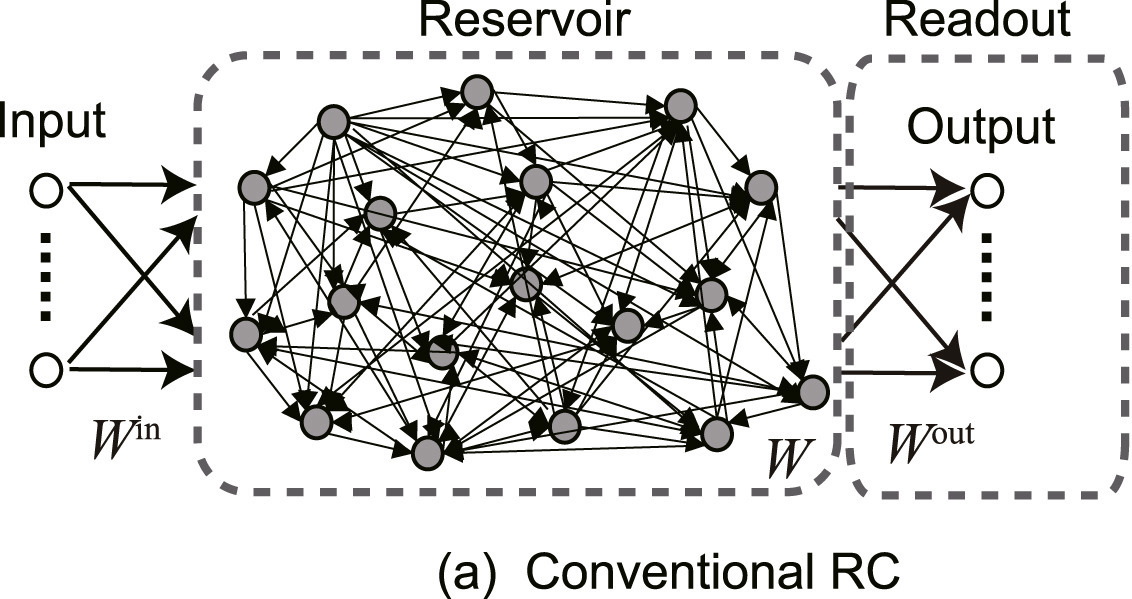
\includegraphics[width=0.79\textwidth]{reservoir}
    \caption[Structure of an echo state network]{Structure of an echo state network. The image is from \citeay{tanaka_recent_2019}.}
    \figlbl{reservoir}
\end{figure}
%
The main distinction between reservoir computing frameworks lies in reservoir design.
An ESN uses the perceptron as the model of neurons and connects them with recurrent connections according to an Erdős–Rényi graph model\sidenote{The Erdős–Rényi model is a model for generating random graphs where all graphs based on a fixed set of vertices and edges are equally likely.} \sidecite{erdos_random_1959}.
LSM, on the other hand, use a spiking neural network instead of a graph of recurrent cells.
The nodes of the spiking neural network are randomly connected.
Thus, every node receives time-varying inputs from other nodes.

The weights of the reservoir connections are randomly assigned and remain unchanged throughout the training process. The readout layer is trained with a supervised learning algorithm such as ridge regression or gradient descent to minimise the discrepancy between predicted and desired outputs.
Thus, the training is very efficient and does not require complex training algorithms, while the system is still able to efficiently process temporal data.

In general, reservoirs are universal approximators and can approximate any non-linear function, given that there are enough neurons in the reservoir.
In principle, the system should be capable of any computation if it has a high enough complexity \cite{adamatzky_reservoir_2018}.
Recently, reservoir computing has become popular in quantum computing \cite{ghosh_quantum_2019, chen_temporal_2020} and for chaotic signal processing \cite{vlachas_backpropagation_2020, krishnagopal_separation_2020}.
However, they are still limited and can only deal well with low-dimensional temporal data. Furthermore, their performance is typically worse than comparable artificial neural networks on most benchmarks \cite{tanaka_recent_2019}.
